% !TeX TXS-program:bibliography = txs:///biber
\documentclass[14pt, russian]{scrartcl}
\let\counterwithout\relax
\let\counterwithin\relax
%\usepackage{lmodern}
\usepackage{float}
\usepackage{xcolor}
\usepackage{extsizes}
\usepackage{subfig}
\usepackage[export]{adjustbox}
\usepackage{tocvsec2} % возможность менять учитываемую глубину разделов в оглавлении
\usepackage[subfigure]{tocloft}
\usepackage[newfloat]{minted}
\captionsetup[listing]{position=top}
\usepackage{subcaption}

\usepackage{fancyvrb}
\usepackage{ulem,bm,mathrsfs,ifsym} %зачеркивания, особо жирный стиль и RSFS начертание
\usepackage{sectsty} % переопределение стилей подразделов
%%%%%%%%%%%%%%%%%%%%%%%

%%% Поля и разметка страницы %%%
\usepackage{pdflscape}                              % Для включения альбомных страниц
\usepackage{geometry}                               % Для последующего задания полей
\geometry{a4paper,tmargin=2cm,bmargin=2cm,lmargin=3cm,rmargin=1cm} % тоже самое, но лучше

%%% Математические пакеты %%%
\usepackage{amsthm,amsfonts,amsmath,amssymb,amscd}  % Математические дополнения от AMS
\usepackage{mathtools}                              % Добавляет окружение multlined
\usepackage[perpage]{footmisc}
%\usepackage{times}

%%%% Установки для размера шрифта 14 pt %%%%
%% Формирование переменных и констант для сравнения (один раз для всех подключаемых файлов)%%
%% должно располагаться до вызова пакета fontspec или polyglossia, потому что они сбивают его работу
%\newlength{\curtextsize}
%\newlength{\bigtextsize}
%\setlength{\bigtextsize}{13pt}
\KOMAoptions{fontsize=14pt}

\makeatletter
\def\showfontsize{\f@size{} point}
\makeatother

%\makeatletter
%\show\f@size                                       % неплохо для отслеживания, но вызывает стопорение процесса, если документ компилируется без команды  -interaction=nonstopmode
%\setlength{\curtextsize}{\f@size pt}
%\makeatother

%шрифт times
\usepackage{tempora} %только для тех, у кого MikTeX последней версии и не ловит pscyr
%\usepackage{pscyr} %для всех нормальных людей
%\setmainfont[Ligatures={TeX,Historic}]{Times New Roman}

   %%% Решение проблемы копирования текста в буфер кракозябрами
%    \input glyphtounicode.tex
%    \input glyphtounicode-cmr.tex %from pdfx package
%    \pdfgentounicode=1
    \usepackage{cmap}                               % Улучшенный поиск русских слов в полученном pdf-файле
    \usepackage[T1]{fontenc}                       % Поддержка русских букв
    \usepackage[utf8]{inputenc}                     % Кодировка utf8
    \usepackage[english, main=russian]{babel}            % Языки: русский, английский
%   \IfFileExists{pscyr.sty}{\usepackage{pscyr}}{}  % Красивые русские шрифты
%\renewcommand{\rmdefault}{ftm}
%%% Оформление абзацев %%%
\usepackage{indentfirst}                            % Красная строка
%\usepackage{eskdpz}

%%% Таблицы %%%
\usepackage{longtable}                              % Длинные таблицы
\usepackage{multirow,makecell,array}                % Улучшенное форматирование таблиц
\usepackage{booktabs}                               % Возможность оформления таблиц в классическом книжном стиле (при правильном использовании не противоречит ГОСТ)

%%% Общее форматирование
\usepackage{soulutf8}                               % Поддержка переносоустойчивых подчёркиваний и зачёркиваний
\usepackage{icomma}                                 % Запятая в десятичных дробях



%%% Изображения %%%
\usepackage{graphicx}                               % Подключаем пакет работы с графикой
\usepackage{wrapfig}

%%% Списки %%%
\usepackage{enumitem}

%%% Подписи %%%
\usepackage{caption}                                % Для управления подписями (рисунков и таблиц) % Может управлять номерами рисунков и таблиц с caption %Иногда может управлять заголовками в списках рисунков и таблиц
%% Использование:
%\begin{table}[h!]\ContinuedFloat - чтобы не переключать счетчик
%\captionsetup{labelformat=continued}% должен стоять до самого caption
%\caption{}
% либо ручками \caption*{Продолжение таблицы~\ref{...}.} :)

%%% Интервалы %%%
\addto\captionsrussian{%
  \renewcommand{\listingname}{Листинг}%
}
%%% Счётчики %%%
\usepackage[figure,table,section]{totalcount}               % Счётчик рисунков и таблиц
\DeclareTotalCounter{lstlisting}
\usepackage{totcount}                               % Пакет создания счётчиков на основе последнего номера подсчитываемого элемента (может требовать дважды компилировать документ)
\usepackage{totpages}                               % Счётчик страниц, совместимый с hyperref (ссылается на номер последней страницы). Желательно ставить последним пакетом в преамбуле

%%% Продвинутое управление групповыми ссылками (пока только формулами) %%%
%% Кодировки и шрифты %%%

%   \newfontfamily{\cyrillicfont}{Times New Roman}
%   \newfontfamily{\cyrillicfonttt}{CMU Typewriter Text}
	%\setmainfont{Times New Roman}
	%\newfontfamily\cyrillicfont{Times New Roman}
	%\setsansfont{Times New Roman}                    %% задаёт шрифт без засечек
%	\setmonofont{Liberation Mono}               %% задаёт моноширинный шрифт
%    \IfFileExists{pscyr.sty}{\renewcommand{\rmdefault}{ftm}}{}
%%% Интервалы %%%
%linespread-реализация ближе к реализации полуторного интервала в ворде.
%setspace реализация заточена под шрифты 10, 11, 12pt, под остальные кегли хуже, но всё же ближе к типографской классике.
\linespread{1.3}                    % Полуторный интервал (ГОСТ Р 7.0.11-2011, 5.3.6)
%\renewcommand{\@biblabel}[1]{#1}

%%% Гиперссылки %%%
\usepackage{hyperref}

%%% Выравнивание и переносы %%%
\sloppy                             % Избавляемся от переполнений
\clubpenalty=10000                  % Запрещаем разрыв страницы после первой строки абзаца
\widowpenalty=10000                 % Запрещаем разрыв страницы после последней строки абзаца

\makeatletter % малые заглавные, small caps shape
\let\@@scshape=\scshape
\renewcommand{\scshape}{%
  \ifnum\strcmp{\f@series}{bx}=\z@
    \usefont{T1}{cmr}{bx}{sc}%
  \else
    \ifnum\strcmp{\f@shape}{it}=\z@
      \fontshape{scsl}\selectfont
    \else
      \@@scshape
    \fi
  \fi}
\makeatother

%%% Подписи %%%
%\captionsetup{%
%singlelinecheck=off,                % Многострочные подписи, например у таблиц
%skip=2pt,                           % Вертикальная отбивка между подписью и содержимым рисунка или таблицы определяется ключом
%justification=centering,            % Центрирование подписей, заданных командой \caption
%}
%%%        Подключение пакетов                 %%%
\usepackage{ifthen}                 % добавляет ifthenelse
%%% Инициализирование переменных, не трогать!  %%%
\newcounter{intvl}
\newcounter{otstup}
\newcounter{contnumeq}
\newcounter{contnumfig}
\newcounter{contnumtab}
\newcounter{pgnum}
\newcounter{bibliosel}
\newcounter{chapstyle}
\newcounter{headingdelim}
\newcounter{headingalign}
\newcounter{headingsize}
\newcounter{tabcap}
\newcounter{tablaba}
\newcounter{tabtita}
%%%%%%%%%%%%%%%%%%%%%%%%%%%%%%%%%%%%%%%%%%%%%%%%%%

%%% Область упрощённого управления оформлением %%%

%% Интервал между заголовками и между заголовком и текстом
% Заголовки отделяют от текста сверху и снизу тремя интервалами (ГОСТ Р 7.0.11-2011, 5.3.5)
\setcounter{intvl}{3}               % Коэффициент кратности к размеру шрифта

%% Отступы у заголовков в тексте
\setcounter{otstup}{0}              % 0 --- без отступа; 1 --- абзацный отступ

%% Нумерация формул, таблиц и рисунков
\setcounter{contnumeq}{1}           % Нумерация формул: 0 --- пораздельно (во введении подряд, без номера раздела); 1 --- сквозная нумерация по всей диссертации
\setcounter{contnumfig}{1}          % Нумерация рисунков: 0 --- пораздельно (во введении подряд, без номера раздела); 1 --- сквозная нумерация по всей диссертации
\setcounter{contnumtab}{1}          % Нумерация таблиц: 0 --- пораздельно (во введении подряд, без номера раздела); 1 --- сквозная нумерация по всей диссертации

%% Оглавление
\setcounter{pgnum}{0}               % 0 --- номера страниц никак не обозначены; 1 --- Стр. над номерами страниц (дважды компилировать после изменения)

%% Библиография
\setcounter{bibliosel}{1}           % 0 --- встроенная реализация с загрузкой файла через движок bibtex8; 1 --- реализация пакетом biblatex через движок biber

%% Текст и форматирование заголовков
\setcounter{chapstyle}{1}           % 0 --- разделы только под номером; 1 --- разделы с названием "Глава" перед номером
\setcounter{headingdelim}{1}        % 0 --- номер отделен пропуском в 1em или \quad; 1 --- номера разделов и приложений отделены точкой с пробелом, подразделы пропуском без точки; 2 --- номера разделов, подразделов и приложений отделены точкой с пробелом.

%% Выравнивание заголовков в тексте
\setcounter{headingalign}{0}        % 0 --- по центру; 1 --- по левому краю

%% Размеры заголовков в тексте
\setcounter{headingsize}{0}         % 0 --- по ГОСТ, все всегда 14 пт; 1 --- пропорционально изменяющийся размер в зависимости от базового шрифта

%% Подпись таблиц
\setcounter{tabcap}{0}              % 0 --- по ГОСТ, номер таблицы и название разделены тире, выровнены по левому краю, при необходимости на нескольких строках; 1 --- подпись таблицы не по ГОСТ, на двух и более строках, дальнейшие настройки:
%Выравнивание первой строки, с подписью и номером
\setcounter{tablaba}{2}             % 0 --- по левому краю; 1 --- по центру; 2 --- по правому краю
%Выравнивание строк с самим названием таблицы
\setcounter{tabtita}{1}             % 0 --- по левому краю; 1 --- по центру; 2 --- по правому краю

%%% Рисунки %%%
\DeclareCaptionLabelSeparator*{emdash}{~--- }             % (ГОСТ 2.105, 4.3.1)
\captionsetup[figure]{labelsep=emdash,font=onehalfspacing,position=bottom}

%%% Таблицы %%%
\ifthenelse{\equal{\thetabcap}{0}}{%
    \newcommand{\tabcapalign}{\raggedright}  % по левому краю страницы или аналога parbox
}

\ifthenelse{\equal{\thetablaba}{0} \AND \equal{\thetabcap}{1}}{%
    \newcommand{\tabcapalign}{\raggedright}  % по левому краю страницы или аналога parbox
}

\ifthenelse{\equal{\thetablaba}{1} \AND \equal{\thetabcap}{1}}{%
    \newcommand{\tabcapalign}{\centering}    % по центру страницы или аналога parbox
}

\ifthenelse{\equal{\thetablaba}{2} \AND \equal{\thetabcap}{1}}{%
    \newcommand{\tabcapalign}{\raggedleft}   % по правому краю страницы или аналога parbox
}

\ifthenelse{\equal{\thetabtita}{0} \AND \equal{\thetabcap}{1}}{%
    \newcommand{\tabtitalign}{\raggedright}  % по левому краю страницы или аналога parbox
}

\ifthenelse{\equal{\thetabtita}{1} \AND \equal{\thetabcap}{1}}{%
    \newcommand{\tabtitalign}{\centering}    % по центру страницы или аналога parbox
}

\ifthenelse{\equal{\thetabtita}{2} \AND \equal{\thetabcap}{1}}{%
    \newcommand{\tabtitalign}{\raggedleft}   % по правому краю страницы или аналога parbox
}

\DeclareCaptionFormat{tablenocaption}{\tabcapalign #1\strut}        % Наименование таблицы отсутствует
\ifthenelse{\equal{\thetabcap}{0}}{%
    \DeclareCaptionFormat{tablecaption}{\tabcapalign #1#2#3}
    \captionsetup[table]{labelsep=emdash}                       % тире как разделитель идентификатора с номером от наименования
}{%
    \DeclareCaptionFormat{tablecaption}{\tabcapalign #1#2\par%  % Идентификатор таблицы на отдельной строке
        \tabtitalign{#3}}                                       % Наименование таблицы строкой ниже
    \captionsetup[table]{labelsep=space}                        % пробельный разделитель идентификатора с номером от наименования
}
\captionsetup[table]{format=tablecaption,singlelinecheck=off,font=onehalfspacing,position=top,skip=-5pt}  % многострочные наименования и прочее
\DeclareCaptionLabelFormat{continued}{Продолжение таблицы~#2}
\setlength{\belowcaptionskip}{.2cm}
\setlength{\intextsep}{0ex}

%%% Подписи подрисунков %%%
\renewcommand{\thesubfigure}{\asbuk{subfigure}}           % Буквенные номера подрисунков
\captionsetup[subfigure]{font={normalsize},               % Шрифт подписи названий подрисунков (не отличается от основного)
    labelformat=brace,                                    % Формат обозначения подрисунка
    justification=centering,                              % Выключка подписей (форматирование), один из вариантов
}
%\DeclareCaptionFont{font12pt}{\fontsize{12pt}{13pt}\selectfont} % объявляем шрифт 12pt для использования в подписях, тут же надо интерлиньяж объявлять, если не наследуется
%\captionsetup[subfigure]{font={font12pt}}                 % Шрифт подписи названий подрисунков (всегда 12pt)

%%% Настройки гиперссылок %%%

\definecolor{linkcolor}{rgb}{0.0,0,0}
\definecolor{citecolor}{rgb}{0,0.0,0}
\definecolor{urlcolor}{rgb}{0,0,0}

\hypersetup{
    linktocpage=true,           % ссылки с номера страницы в оглавлении, списке таблиц и списке рисунков
%    linktoc=all,                % both the section and page part are links
%    pdfpagelabels=false,        % set PDF page labels (true|false)
    plainpages=true,           % Forces page anchors to be named by the Arabic form  of the page number, rather than the formatted form
    colorlinks,                 % ссылки отображаются раскрашенным текстом, а не раскрашенным прямоугольником, вокруг текста
    linkcolor={linkcolor},      % цвет ссылок типа ref, eqref и подобных
    citecolor={citecolor},      % цвет ссылок-цитат
    urlcolor={urlcolor},        % цвет гиперссылок
    pdflang={ru},
}
\urlstyle{same}
%%% Шаблон %%%
%\DeclareRobustCommand{\todo}{\textcolor{red}}       % решаем проблему превращения названия цвета в результате \MakeUppercase, http://tex.stackexchange.com/a/187930/79756 , \DeclareRobustCommand protects \todo from expanding inside \MakeUppercase
\setlength{\parindent}{2.5em}                       % Абзацный отступ. Должен быть одинаковым по всему тексту и равен пяти знакам (ГОСТ Р 7.0.11-2011, 5.3.7).

%%% Списки %%%
% Используем дефис для ненумерованных списков (ГОСТ 2.105-95, 4.1.7)
%\renewcommand{\labelitemi}{\normalfont\bfseries~{---}}
\renewcommand{\labelitemi}{\bfseries~{---}}
\setlist{nosep,%                                    % Единый стиль для всех списков (пакет enumitem), без дополнительных интервалов.
    labelindent=\parindent,leftmargin=*%            % Каждый пункт, подпункт и перечисление записывают с абзацного отступа (ГОСТ 2.105-95, 4.1.8)
}
%%%%%%%%%%%%%%%%%%%%%%
%\usepackage{xltxtra} % load xunicode

\usepackage{ragged2e}
\usepackage[explicit]{titlesec}
\usepackage{placeins}
\usepackage{xparse}
\usepackage{csquotes}

\usepackage{listingsutf8}
\usepackage{url} %пакеты расширений
\usepackage{algorithm, algorithmicx}
\usepackage[noend]{algpseudocode}
\usepackage{blkarray}
\usepackage{chngcntr}
\usepackage{tabularx}
\usepackage[backend=biber,
    bibstyle=gost-numeric,
    citestyle=nature]{biblatex}
\newcommand*\template[1]{\text{<}#1\text{>}}
\addbibresource{biblio.bib}

\titleformat{name=\section,numberless}[block]{\normalfont\large\centering}{}{0em}{#1}
\titleformat{\section}[block]{\normalfont\large\bfseries\raggedright}{}{0em}{\thesection\hspace{0.25em}#1}
\titleformat{\subsection}[block]{\normalfont\large\bfseries\raggedright}{}{0em}{\thesubsection\hspace{0.25em}#1}
\titleformat{\subsubsection}[block]{\normalfont\large\bfseries\raggedright}{}{0em}{\thesubsubsection\hspace{0.25em}#1}

\let\Algorithm\algorithm
\renewcommand\algorithm[1][]{\Algorithm[#1]\setstretch{1.5}}
%\renewcommand{\listingscaption}{Листинг}

\usepackage{pifont}
\usepackage{calc}
\usepackage{suffix}
\usepackage{csquotes}
\DeclareQuoteStyle{russian}
    {\guillemotleft}{\guillemotright}[0.025em]
    {\quotedblbase}{\textquotedblleft}
\ExecuteQuoteOptions{style=russian}
\newcommand{\enq}[1]{\enquote{#1}}
\newcommand{\eng}[1]{\begin{english}#1\end{english}}
% Подчиненные счетчики в окружениях http://old.kpfu.ru/journals/izv_vuz/arch/sample1251.tex
\newcounter{cTheorem}
\newcounter{cDefinition}
\newcounter{cConsequent}
\newcounter{cExample}
\newcounter{cLemma}
\newcounter{cConjecture}
\newtheorem{Theorem}{Теорема}[cTheorem]
\newtheorem{Definition}{Определение}[cDefinition]
\newtheorem{Consequent}{Следствие}[cConsequent]
\newtheorem{Example}{Пример}[cExample]
\newtheorem{Lemma}{Лемма}[cLemma]
\newtheorem{Conjecture}{Гипотеза}[cConjecture]

\renewcommand{\theTheorem}{\arabic{Theorem}}
\renewcommand{\theDefinition}{\arabic{Definition}}
\renewcommand{\theConsequent}{\arabic{Consequent}}
\renewcommand{\theExample}{\arabic{Example}}
\renewcommand{\theLemma}{\arabic{Lemma}}
\renewcommand{\theConjecture}{\arabic{Conjecture}}
%\makeatletter
\NewDocumentCommand{\Newline}{}{\text{\\}}
\newcommand{\sequence}[2]{\ensuremath \left(#1,\ \dots,\ #2\right)}

\definecolor{mygreen}{rgb}{0,0.6,0}
\definecolor{mygray}{rgb}{0.5,0.5,0.5}
\definecolor{mymauve}{rgb}{0.58,0,0.82}
\renewcommand{\listalgorithmname}{Список алгоритмов}
\floatname{algorithm}{Листинг}
\renewcommand{\lstlistingname}{Листинг}
\renewcommand{\thealgorithm}{\arabic{algorithm}}

\newcommand{\refAlgo}[1]{(листинг \ref{#1})}
\newcommand{\refImage}[1]{(рисунок \ref{#1})}

\renewcommand{\theenumi}{\arabic{enumi}.}% Меняем везде перечисления на цифра.цифра
\renewcommand{\labelenumi}{\arabic{enumi}.}% Меняем везде перечисления на цифра.цифра
\renewcommand{\theenumii}{\arabic{enumii}}% Меняем везде перечисления на цифра.цифра
\renewcommand{\labelenumii}{(\arabic{enumii})}% Меняем везде перечисления на цифра.цифра
\renewcommand{\theenumiii}{\roman{enumiii}}% Меняем везде перечисления на цифра.цифра
\renewcommand{\labelenumiii}{(\roman{enumiii})}% Меняем везде перечисления на цифра.цифра
%\newfontfamily\AnkaCoder[Path=src/fonts/]{AnkaCoder-r.ttf}
\renewcommand{\labelitemi}{---}
\renewcommand{\labelitemii}{---}

%\usepackage{courier}

\makeatletter
\def\p@subsection{}
\def\p@subsubsection{\thesection\,\thesubsection\,}
\makeatother
\newcommand{\prog}[1]{{\ttfamily\small#1}}

\newcommand{\anonsection}[1]{\cleardoublepage
\phantomsection
\addcontentsline{toc}{section}{\protect\numberline{}#1}
\section*{#1}\vspace*{2.5ex} % По госту положены 3 пустые строки после заголовка ненумеруемого раздела
}
\newcommand{\sectionbreak}{\clearpage}
\renewcommand{\sectionfont}{\normalsize} % Сбиваем стиль оглавления в стандартный
\renewcommand{\cftsecleader}{\cftdotfill{\cftdotsep}} % Точки в оглавлении напротив разделов

\renewcommand{\cftsecfont}{\normalfont\large} % Переключение на times в содержании
\renewcommand{\cftsubsecfont}{\normalfont\large} % Переключение на times в содержании

\usepackage{caption}
%\captionsetup[table]{justification=raggedleft}
%\captionsetup[figure]{justification=centering,labelsep=endash}
\usepackage{amsmath}    % \bar    (матрицы и проч. ...)
\usepackage{amsfonts}   % \mathbb (символ для множества действительных чисел и проч. ...)
\usepackage{mathtools}  % \abs, \norm
    \DeclarePairedDelimiter\abs{\lvert}{\rvert} % операция модуля
    \DeclarePairedDelimiter\norm{\lVert}{\rVert} % операция нормы
\DeclareTextCommandDefault{\textvisiblespace}{%
  \mbox{\kern.06em\vrule \@height.3ex}%
  \vbox{\hrule \@width.3em}%
  \hbox{\vrule \@height.3ex}}
\newsavebox{\spacebox}
\begin{lrbox}{\spacebox}
\verb*! !
\end{lrbox}
\newcommand{\aspace}{\usebox{\spacebox}}
\DeclareTotalCounter{listing}

\makeatletter
\renewcommand*{\p@subsubsection}{}
\makeatother

\newenvironment{longlisting}{\captionsetup{type=listing}}{}

\begin{document}
\sloppy

\begin{titlepage}
\begin{center}

{\large \textbf{ФЕДЕРАЛЬНОЕ ГОСУДАРСТВЕННОЕ АВТОНОМНОЕ}}\\[0.3cm]
{\large \textbf{ОБРАЗОВАТЕЛЬНОЕ УЧРЕЖДЕНИЕ ВЫСШЕГО ОБРАЗОВАНИЯ}}\\[0.5cm]

% \includegraphics[width=0.2\textwidth]{emblem.png}\\[0.5cm]

% {\large \textbf{МОСКОВСКИЙ ПОЛИТЕХНИЧЕСКИЙ УНИВЕРСИТЕТ}}\\[0.5cm]

% {\large Факультет информационных технологий}\\[0.3cm]
% {\large Кафедра Информатики и информационных технологий}\\[1cm]

% {\large направление подготовки 09.04.02 «Информационные системы и}\\
% {\large технологии»,}\\[0.3cm]
% {\large профиль «Мобильные технологии»}\\[2cm]

% {\Large \textbf{КУРСОВАЯ РАБОТА}}\\[1cm]

% {\large \textbf{Дисциплина:} «Мобильные операционные системы»}\\[3cm]

% \end{center}

% \begin{flushright}
% \begin{tabular}{ll}
% {\large \textbf{Выполнил:} студент группы 211-362}\\
% {\large Владиславов А.А.}\\[0.5cm]
% {\large \textbf{Дата, подпись} \rule{5cm}{0.4pt} \rule{5cm}{0.4pt}}\\
% {\scriptsize \hspace*{7.5cm}(Дата) \hspace{3.5cm}(Подпись)}\\[1cm]
% {\large \textbf{Проверил:} к.т.н., доцент}\\
% {\large Кузнецов И.А.}\\[0.5cm]
% {\large \textbf{Дата, подпись} \rule{5cm}{0.4pt} \rule{5cm}{0.4pt}}\\
% {\scriptsize \hspace*{7.5cm}(Дата) \hspace{3.5cm}(Подпись)}\\[0.3cm]
% {\large \hspace*{11cm}(Оценка)}
% \end{tabular}
% \end{flushright}

% \vspace{1cm}
% {\large \textbf{Замечания:}}\\[0.3cm]
% \rule{\textwidth}{0.4pt}\\[0.3cm]
% \rule{\textwidth}{0.4pt}

% \vfill

% \begin{center}
% {\large \textbf{Москва}}\\
% {\large \textbf{2024}}
\end{center}

\end{titlepage}
%\renewcommand{\ttdefault}{pcr}

\setlength{\tabcolsep}{3pt}
\newpage
\setcounter{page}{2}
%----------------------------------------------------------------------------
%                  ОТСЮДА --- СОБСТВЕННО ТЕКСТ
%----------------------------------------------------------------------------
\renewcommand\contentsname{\hfill{\normalfont{СОДЕРЖАНИЕ}}\hfill}  %Оглавление
\tableofcontents
\newpage


\section{Постановка исследовательской задачи}

Целью курсовой работы является проведение сравнительного анализа архитектурных подходов для создания мультиплатформенных приложений на Kotlin Multiplatform (KMP) с особым акцентом на интеграцию с нативной платформой iOS. В рамках исследования будут рассмотрены и сопоставлены как традиционные паттерны iOS-разработки (MVVM, Redux), так и современные KMP-ориентированные стеки (MVIKotlin с Decompose, MVVM из пакета Jetpack ViewModel). Основная задача — выявить наиболее эффективное и удобное решение для проекта, где iOS является одной из ключевых платформ.

Для достижения поставленной цели предполагается решить следующие задачи:

\begin{enumerate}
    \item Проанализировать теоретические основы и практическое применение архитектурных паттернов MVVM и Redux в контексте нативной iOS-разработки.
    \item Исследовать доступные архитектурные решения для Kotlin Multiplatform, уделив внимание подходам к управлению состоянием (MVI, MVVM) и навигации (Decompose, Jetpack Navigation).
    \item Определить ключевые критерии для сравнения подходов: сложность интеграции со SwiftUI, объем переиспользуемого кода, простота тестирования, количество шаблонного кода и общий опыт разработчика.
    \item На основе теоретического анализа и сформулированных критериев выбрать и обосновать наиболее подходящий архитектурный стек для дальнейшей реализации.
    \item Разработать прототип приложения, чтобы на практике проверить гипотезы и оценить выбранную архитектуру.
    \item Сформулировать выводы и рекомендации по применению исследуемых подходов в проектах на KMP с фокусом на iOS.
\end{enumerate}

Данная работа является актуальной, поскольку технология Kotlin Multiplatform, несмотря на растущую популярность, еще не имеет устоявшихся архитектурных стандартов, в особенности для реализации навигации и управления состоянием. Это создает значительные трудности для разработчиков, особенно для тех, кто переходит с нативной iOS-разработки и оказывается перед выбором: адаптировать привычные паттерны, такие как MVVM, или осваивать новые, KMP-специфичные библиотеки, например, MVIKotlin и Decompose. Отсутствие четких сравнительных анализов и практических рекомендаций усложняет принятие архитектурных решений и повышает риски при старте новых проектов. Таким образом, систематизация и сравнительный анализ ключевых архитектурных подходов для KMP-приложений с фокусом на iOS представляет собой важную практическую задачу.


\section{Теоретический обзор}

\subsection{Нативные подходы в iOS разработке}

\subsubsection{Паттерн Model-View-ViewModel (MVVM)}

Model-View-ViewModel (MVVM) — это архитектурный паттерн проектирования, который упрощает разделение разработки графического интерфейса пользователя (UI) от бизнес-логики или логики представления. Он был создан как ответ на недостатки таких паттернов, как MVC и MVP, и получил широкое распространение в разработке под iOS с появлением фреймворков Combine и SwiftUI, которые обеспечивают нативную поддержку для связывания данных (data binding).

Основные компоненты паттерна:
\begin{itemize}
    \item Model (Модель) — представляет данные и бизнес-логику приложения. Она не имеет прямого знания о \texttt{ViewModel} и \texttt{View}.
    \item View (Представление) — отвечает за отображение данных пользователю и передачу его действий в \texttt{ViewModel}. В SwiftUI \texttt{View} декларативно описывает UI и подписывается на изменения в `ViewModel`.
    \item ViewModel (Модель представления) — выступает посредником между \texttt{Model} и \texttt{View}. Она получает данные из \texttt{Model}, обрабатывает их и предоставляет в формате, удобном для отображения в \texttt{View}. \texttt{ViewModel} ничего не знает о конкретной реализации \texttt{View}.
\end{itemize}

Ключевой особенностью MVVM является механизм связывания данных (Data Binding). В экосистеме Apple он реализуется через фреймворк Combine, который позволяет \texttt{View} автоматически обновляться при изменении данных в \texttt{ViewModel}.

Пример реализации на Swift и SwiftUI:

В качестве примера рассмотрим экран, отображающий информацию о пользователе.

\begin{enumerate}
    \item Model

    Это простая структура данных, представляющая бизнес-сущность. Пример представлен на листинге \ref{lst:swift_mvvm_model}

    \begin{listing}[H]
    \begin{minted}[frame=single,framesep=2mm,baselinestretch=1.2,fontsize=\small,linenos,breaklines]{swift}
    struct User {
        let name: String
        let age: Int
    }
    \end{minted}
    \caption{Model: простая структура данных}
    \label{lst:swift_mvvm_model}
    \end{listing}

    \item ViewModel

    \texttt{ViewModel} инкапсулирует логику представления, получая данные из \texttt{Model} и подготавливая их для \texttt{View}, как представлено на листинге \ref{lst:swith_mvvm_vm}.

    \begin{listing}[H]
    \begin{minted}[frame=single,framesep=2mm,baselinestretch=1.2,fontsize=\small,linenos,breaklines]{swift}
    import Combine

    class UserViewModel: ObservableObject {
        @Published var userName: String = "Загрузка..."
        @Published var isPremium: Bool = false
        private var user: User?

        func fetchUser() {
            // Имитация асинхронной загрузки
            DispatchQueue.main.asyncAfter(deadline: .now() + 1) {
                self.user = User(name: "Иван", age: 30)
                self.userName = self.user?.name ?? ""
                self.isPremium = (self.user?.age ?? 0) > 25
            }
        }
    }
    \end{minted}
    \caption{ViewModel: Управляет логикой представления}
    \label{lst:swith_mvvm_vm}
    \end{listing}

    \item View

    \texttt{View} декларативно описывает интерфейс и подписывается на изменения в \texttt{ViewModel}, как представлено в листинге \ref{lst:swith_mvvm_view}.

    \begin{listing}[H]
    \begin{minted}[frame=single,framesep=2mm,baselinestretch=1.2,fontsize=\small,linenos,breaklines]{swift}
import SwiftUI

struct UserView: View {
    @StateObject private var viewModel = UserViewModel()

    var body: some View {
        VStack(spacing: 16) {
            Text(viewModel.userName)
                .font(.title)
            if viewModel.isPremium {
                Text("Премиум-пользователь")
                    .foregroundColor(.green)
            }
        }
        .onAppear(perform: viewModel.fetchUser)
    }
}
    \end{minted}
    \caption{View: Отображает данные и взаимодействует с пользователем}
    \label{lst:swith_mvvm_view}
    \end{listing}

\end{enumerate}

Преимущества MVVM:

\begin{itemize}
    \item Разделение логики: Четко отделяет логику представления (\texttt{ViewModel}) от пользовательского интерфейса (\texttt{View}), что делает код более структурированным и легким для понимания.
    \item Высокая тестируемость: Так как \texttt{ViewModel} не имеет прямой зависимости от UI-компонентов, ее логику можно легко покрыть автоматизированными юнит-тестами.
    \item Связывание данных (Data Binding): Нативная поддержка со стороны SwiftUI и Combine позволяет автоматически синхронизировать данные между \texttt{ViewModel} и \texttt{View}, что сокращает количество шаблонного кода для обновления UI.
\end{itemize}

Недостатки:
\begin{itemize}
    \item Проблема масштабирования: На сложных экранах, где множество компонентов взаимодействуют друг с другом, \texttt{ViewModel} может стать слишком громоздкой (т.н. "Massive ViewModel"). Это затрудняет поддержку и навигацию по коду.
    \item Синхронизация состояния: При дроблении логики на несколько \texttt{ViewModel} для одного экрана возникает проблема синхронизации состояния и обмена данными между ними, что усложняет поток данных.
    \item Неявный поток данных: В отличие от однонаправленных потоков (как в Redux/MVI), логика обработки действий пользователя и изменения состояния может быть разбросана по разным методам \texttt{ViewModel}, что делает поток данных менее предсказуемым и сложным для отладки.
\end{itemize}

\subsubsection{Паттерн Redux}

Redux — это архитектурный паттерн и библиотека для управления состоянием приложения, основанная на принципах функционального программирования. Хотя он зародился в экосистеме JavaScript (React), его концепции были успешно адаптированы и для нативной iOS-разработки, часто с использованием таких библиотек, как ReSwift или The Composable Architecture (TCA), которая во многом следует идеям Redux.

Ключевые принципы Redux:
\begin{itemize}
    \item Единый источник истины (Single Source of Truth): Состояние всего приложения хранится в одном объекте — \texttt{Store}. Это упрощает отладку и инспектирование состояния.
    \item Состояние только для чтения (State is read-only): Единственный способ изменить состояние — это отправить (dispatch) \texttt{Action} (действие), которое является простым объектом, описывающим намерение изменения.
    \item Изменения вносятся чистыми функциями: Для обработки \texttt{Action} и обновления состояния используются \texttt{Reducers} (редьюсеры) — чистые функции, которые принимают текущее состояние и \texttt{Action}, а затем возвращают новое состояние.
\end{itemize}

Пример реализации на Swift (концептуальный):

Рассмотрим простой счетчик.

\begin{enumerate}
    \item State, Actions и Reducer

    Определим состояние, возможные действия и чистую функцию для их обработки, как представлено в листинге \ref{lst:swift_redux_state}.

    \begin{listing}[H]
    \begin{minted}[frame=single,framesep=2mm,baselinestretch=1.2,fontsize=\small,linenos,breaklines]{swift}
    struct CounterState {
        var count: Int = 0
    }

    enum CounterAction {
        case increment
        case decrement
    }

    func counterReducer(state: inout CounterState, action: CounterAction) {
        switch action {
        case .increment: state.count += 1
        case .decrement: state.count -= 1
        }
    }
    \end{minted}
    \caption{State, Actions и Reducer: Определение состояния и действий}
    \label{lst:swift_redux_state}
    \end{listing}

    \item Store

    \texttt{Store} управляет состоянием и является единственным источником истины, как показано в листинге \ref{lst:swift_redux_store}.

    \begin{listing}[H]
    \begin{minted}[frame=single,framesep=2mm,baselinestretch=1.2,fontsize=\small,linenos,breaklines]{swift}
    import Combine

    class Store<State, Action>: ObservableObject {
        @Published private(set) var state: State
        private var reducer: (inout State, Action) -> Void

        init(initialState: State, reducer: @escaping (inout State, Action) -> Void) {
            self.state = initialState
            self.reducer = reducer
        }

        func dispatch(_ action: Action) {
            reducer(&state, action)
        }
    }
    \end{minted}
    \caption{Store: Управление состоянием}
    \label{lst:swift_redux_store}
    \end{listing}

    \item View

    \texttt{View} отображает состояние из \texttt{Store} и отправляет действия при взаимодействии, как представлено в листинге \ref{lst:swift_redux_view}.

    \begin{listing}[H]
    \begin{minted}[frame=single,framesep=2mm,baselinestretch=1.2,fontsize=\small,linenos,breaklines]{swift}
    import SwiftUI

    struct CounterView: View {
        @StateObject private var store = Store(
            initialState: CounterState(),
            reducer: counterReducer
        )

        var body: some View {
            VStack {
                Text("Count: \(store.state.count)")
                HStack {
                    Button("Increment") { store.dispatch(.increment) }
                    Button("Decrement") { store.dispatch(.decrement) }
                }
            }
        }
    }
    \end{minted}
    \caption{View: Отображение состояния и отправка действий}
    \label{lst:swift_redux_view}
    \end{listing}
\end{enumerate}

Преимущества Redux:
\begin{itemize}
    \item Предсказуемость: Однонаправленный поток данных делает логику изменения состояния строгой и легкой для отслеживания.
    \item Централизованное состояние: Упрощает передачу данных между разными частями приложения без необходимости пробрасывать их через множество слоев.
    \item Отличные инструменты для отладки: Возможность "путешествия во времени" (time travel debugging), логирование всех действий.
\end{itemize}

Недостатки:
\begin{itemize}
    \item Многословность (Boilerplate): Требует описания \texttt{State}, \texttt{Actions} и \texttt{Reducer}, что может быть избыточным для простых экранов.
    \item Сложен для понимания: Требует понимания принципов функционального программирования.
    \item Производительность: В очень больших приложениях с частыми обновлениями состояния могут возникнуть проблемы с производительностью, если не применять оптимизации.
\end{itemize}

\subsection{Архитектурные подходы в Kotlin Multiplatform}

\subsubsection{Адаптация MVVM с Jetpack ViewModel}

Стремление использовать привычный паттерн MVVM в KMP-проектах привело к появлению различных решений. Изначально \texttt{ViewModel} из Android Jetpack не была мультиплатформенной, что заставляло разработчиков создавать собственные реализации или использовать сторонние библиотеки (например, \texttt{moko-mvvm}).

Однако с недавнего времени Google официально поддерживает Jetpack ViewModel в Kotlin Multiplatform (\texttt{androidx.lifecycle:lifecycle-viewmodel-compose}). Это позволяет определять \texttt{ViewModel} в общем коде (\texttt{commonMain}), переиспользуя логику представления на всех платформах. На Android \texttt{ViewModel} автоматически интегрируется с жизненным циклом компонентов, а на iOS требует ручного создания и удержания.

Пример реализации:

\begin{enumerate}
    \item ViewModel в общем коде (\texttt{commonMain})

    \texttt{ViewModel} определяется в общем модуле и использует \texttt{StateFlow} для предоставления состояния, как показано в листинге \ref{lst:kotlin_mvvm_vm}.

    \begin{listing}[H]
    \begin{minted}[frame=single,framesep=2mm,baselinestretch=1.2,fontsize=\small,linenos,breaklines]{kotlin}
    import androidx.lifecycle.ViewModel
    import androidx.lifecycle.viewModelScope
    import kotlinx.coroutines.flow.MutableStateFlow
    import kotlinx.coroutines.flow.asStateFlow
    import kotlinx.coroutines.launch

    class GreetingViewModel : ViewModel() {
        private val _greetingText = MutableStateFlow("Загрузка...")
        val greetingText = _greetingText.asStateFlow()

        fun greet() {
            viewModelScope.launch {
                _greetingText.value = "Привет из KMP ViewModel!"
            }
        }
    }
    \end{minted}
    \caption{ViewModel: Определение в общем коде}
    \label{lst:kotlin_mvvm_vm}
    \end{listing}

    \item Интеграция с iOS и SwiftUI

    На стороне iOS для корректной интеграции со SwiftUI и подписки на \texttt{StateFlow} обычно создается класс-обертка, который является \texttt{ObservableObject}, как представлено в листинге \ref{lst:swift_mvvm_integration}.

    \begin{listing}[H]
    \begin{minted}[frame=single,framesep=2mm,baselinestretch=1.2,fontsize=\small,linenos,breaklines]{swift}
    import Foundation
    import Combine
    import shared

    class GreetingIOSViewModel: ObservableObject {
        @Published var text: String = "..."

        private let kmpViewModel = GreetingViewModel()
        private var cancellable: AnyCancellable? = nil

        init() {
            // Установка подписки на StateFlow
            self.cancellable = kmpViewModel.greetingText
                .toPublisher()
                .receive(on: DispatchQueue.main)
                .sink { self.text = $0 }
        }

        func greet() {
            kmpViewModel.greet()
        }
    }
    \end{minted}
    \caption{Интеграция с iOS: Класс-обертка для ViewModel}
    \label{lst:swift_mvvm_integration}
    \end{listing}

    \item View в SwiftUI

    \texttt{View} работает уже с iOS-специфичной \texttt{ViewModel}, как показано в листинге \ref{lst:swift_mvvm_view}.

    \begin{listing}[H]
    \begin{minted}[frame=single,framesep=2mm,baselinestretch=1.2,fontsize=\small,linenos,breaklines]{swift}
    import SwiftUI

    struct ContentView: View {
        @StateObject private var viewModel = GreetingIOSViewModel()

        var body: some View {
            VStack {
                Text(viewModel.text)
                Button("Обновить", action: viewModel.greet)
            }
            .onAppear(perform: viewModel.greet)
        }
    }
    \end{minted}
    \caption{View: Работа с iOS-специфичной ViewModel}
    \label{lst:swift_mvvm_view}
    \end{listing}
\end{enumerate}

Преимущества:
\begin{itemize}
    \item Официальная поддержка: Подход поддерживается Google, что гарантирует его развитие и стабильность.
    \item Привычность для Android-разработчиков: Позволяет использовать знакомые концепции \texttt{ViewModel} и \texttt{viewModelScope}.
    \item Разделение логики: Сохраняется ключевое преимущество MVVM — отделение логики от UI.
\end{itemize}

Недостатки:
\begin{itemize}
    \item Шаблонный код на iOS: Требуется создавать классы-обертки для каждой \texttt{ViewModel}, чтобы связать их со SwiftUI.
    \item Отсутствие управления навигацией: Данный подход решает только проблему \texttt{ViewModel}, но не предлагает общего решения для навигации между экранами.
    \item Управление жизненным циклом на iOS: Необходимо вручную создавать и удерживать \texttt{ViewModel} на стороне iOS, в то время как на Android это происходит автоматически.
\end{itemize}

\subsubsection{MVIKotlin с Decompose}

MVIKotlin — это библиотека для Kotlin Multiplatform, реализующая архитектурный паттерн Model-View-Intent (MVI). В сочетании с Decompose — библиотекой для управления навигацией и жизненным циклом компонентов — она предоставляет полноценное решение для создания мультиплатформенных приложений.

Ключевые концепции MVI:
\begin{itemize}
    \item Model — состояние компонента
    \item View — UI-слой, отображающий состояние
    \item Intent — действия пользователя или системы
    \item Store — компонент, обрабатывающий Intent'ы и обновляющий состояние
\end{itemize}

Пример реализации:

\begin{enumerate}
    \item Определение состояния и действий

    Определим состояние и возможные действия, как показано в листинге \ref{lst:kotlin_mvi_state}.

    \begin{listing}[H]
    \begin{minted}[frame=single,framesep=2mm,baselinestretch=1.2,fontsize=\small,linenos,breaklines]{kotlin}
    data class CounterState(
        val count: Int = 0
    )

    sealed class CounterIntent {
        object Increment : CounterIntent()
        object Decrement : CounterIntent()
    }
    \end{minted}
    \caption{Определение состояния и действий}
    \label{lst:kotlin_mvi_state}
    \end{listing}

    \item Создание Store

    Создадим Store для обработки действий и обновления состояния, как представлено в листинге \ref{lst:kotlin_mvi_store}.

    \begin{listing}[H]
    \begin{minted}[frame=single,framesep=2mm,baselinestretch=1.2,fontsize=\small,linenos,breaklines]{kotlin}
    import com.arkivanov.mvikotlin.core.store.Store
    import com.arkivanov.mvikotlin.main.store.DefaultStoreFactory

    class CounterStore(
        storeFactory: DefaultStoreFactory
    ) : Store<CounterIntent, CounterState, Nothing> by storeFactory.create(
        name = "CounterStore",
        initialState = CounterState(),
        reducer = { intent, state ->
            when (intent) {
                is CounterIntent.Increment -> state.copy(count = state.count + 1)
                is CounterIntent.Decrement -> state.copy(count = state.count - 1)
            }
        }
    )
    \end{minted}
    \caption{Создание Store}
    \label{lst:kotlin_mvi_store}
    \end{listing}

    \item Создание компонента с Decompose

    Создадим компонент, который будет управлять жизненным циклом и состоянием, как показано в листинге \ref{lst:kotlin_mvi_component}.

    \begin{listing}[H]
    \begin{minted}[frame=single,framesep=2mm,baselinestretch=1.2,fontsize=\small,linenos,breaklines]{kotlin}
    import com.arkivanov.decompose.ComponentContext
    import com.arkivanov.essenty.lifecycle.doOnDestroy

    class CounterComponent(
        componentContext: ComponentContext,
        private val storeFactory: DefaultStoreFactory
    ) : ComponentContext by componentContext {
        private val store = CounterStore(storeFactory)

        val state = store.state

        fun increment() {
            store.accept(CounterIntent.Increment)
        }

        fun decrement() {
            store.accept(CounterIntent.Decrement)
        }

        init {
            lifecycle.doOnDestroy {
                store.dispose()
            }
        }
    }
    \end{minted}
    \caption{Создание компонента с Decompose}
    \label{lst:kotlin_mvi_component}
    \end{listing}

    \item Интеграция с iOS и SwiftUI

    Для интеграции Decompose со SwiftUI возможно использовать универсальную обертку, которая превращает \texttt{Value} из мира Decompose в \texttt{ObservableObject} для мира SwiftUI. Это позволяет избежать написания повторяющегося кода для каждого экрана. Пример представлен в листингах \ref{lst:swift_mvi_obsvalue}, \ref{lst:swift_mvi_view}.

    \begin{listing}[H]
    \begin{minted}[frame=single,framesep=2mm,baselinestretch=1.2,fontsize=\small,linenos,breaklines]{swift}
import SwiftUI
import shared

class ObservableValue<T>: ObservableObject {
    @Published var value: T
    private var cancellation: Cancellation?

    init(_ value: Value<T>) {
        self.value = value.value
        self.cancellation = value.subscribe { [weak self] in
            self?.value = $0
        }
    }

    deinit {
        cancellation?.cancel()
    }
}
    \end{minted}
    \caption{Универсальная обертка ObservableValue}
    \label{lst:swift_mvi_obsvalue}
    \end{listing}

    \begin{listing}[H]
    \begin{minted}[frame=single,framesep=2mm,baselinestretch=1.2,fontsize=\small,linenos,breaklines]{swift}
struct CounterView: View {
    @StateObject private var model: ObservableValue<CounterState>

    private let component: CounterComponent

    init(_ component: CounterComponent) {
        self.component = component
        _model = StateObject(wrappedValue: ObservableValue(component.state))
    }

    var body: some View {
        VStack(spacing: 16) {
            Text("Count: \(model.value.count)")
                .font(.title)

            HStack(spacing: 24) {
                Button("Increment") { component.increment() }
                Button("Decrement") { component.decrement() }
            }
        }
    }
}
    \end{minted}
    \caption{SwiftUI View, использующее обертку}
    \label{lst:swift_mvi_view}
    \end{listing}
\end{enumerate}

Преимущества MVIKotlin с Decompose:
\begin{itemize}
    \item Единый подход к навигации: Decompose предоставляет унифицированное решение для управления навигацией на всех платформах.
    \item Предсказуемый поток данных: Однонаправленный поток данных делает поведение приложения более предсказуемым и тестируемым.
    \item Мультиплатформенность: Все компоненты определены в общем коде, что обеспечивает максимальное переиспользование.
    \item Управление жизненным циклом: Decompose автоматически управляет жизненным циклом компонентов на всех платформах.
\end{itemize}

Недостатки:
\begin{itemize}
    \item Сложность интеграции: Требует более глубокого понимания архитектуры и дополнительных настроек по сравнению с MVVM.
    \item Объем шаблонного кода: Необходимость определения состояний, интентов и редьюсеров для каждого компонента может привести к увеличению объема кода.
    \item Необходимо обучение: Разработчикам, привыкшим к традиционным паттернам, может потребоваться время для освоения MVI и Decompose.
\end{itemize}

\section{Детали реализации}

В рамках практической части работы было разработано мультиплатформенное приложение на Kotlin Multiplatform, демонстрирующее получение, отображение и навигацию по данным, полученным из открытого API.

\subsection{Функциональность}

Приложение реализует базовый сценарий взаимодействия с удаленным сервером и предоставляет следующий функционал:

\begin{enumerate}
    \item Отображение списка персонажей: При запуске приложения открывается главный экран, на котором в виде списка отображаются персонажи, загруженные из Star Wars API (SWAPI). Реализована пагинация для постепенной подгрузки данных при прокрутке списка (см. рисунок \ref{fig:list_screen}).
    \item Просмотр детальной информации: При нажатии на элемент списка происходит переход на экран с подробной информацией о выбранном персонаже (см. рисунок \ref{fig:details_screen}).
    \item Обработка состояний: В приложении реализована обработка состояний загрузки (рисунок \ref{fig:loading_screen}) и ошибок (рисунок ~\ref{fig:error_screen}) как для списка, так и для экрана с детальной информацией, что обеспечивает корректное отображение UI в различных сценариях.
\end{enumerate}

\begin{figure}[!htb]
    \centering
    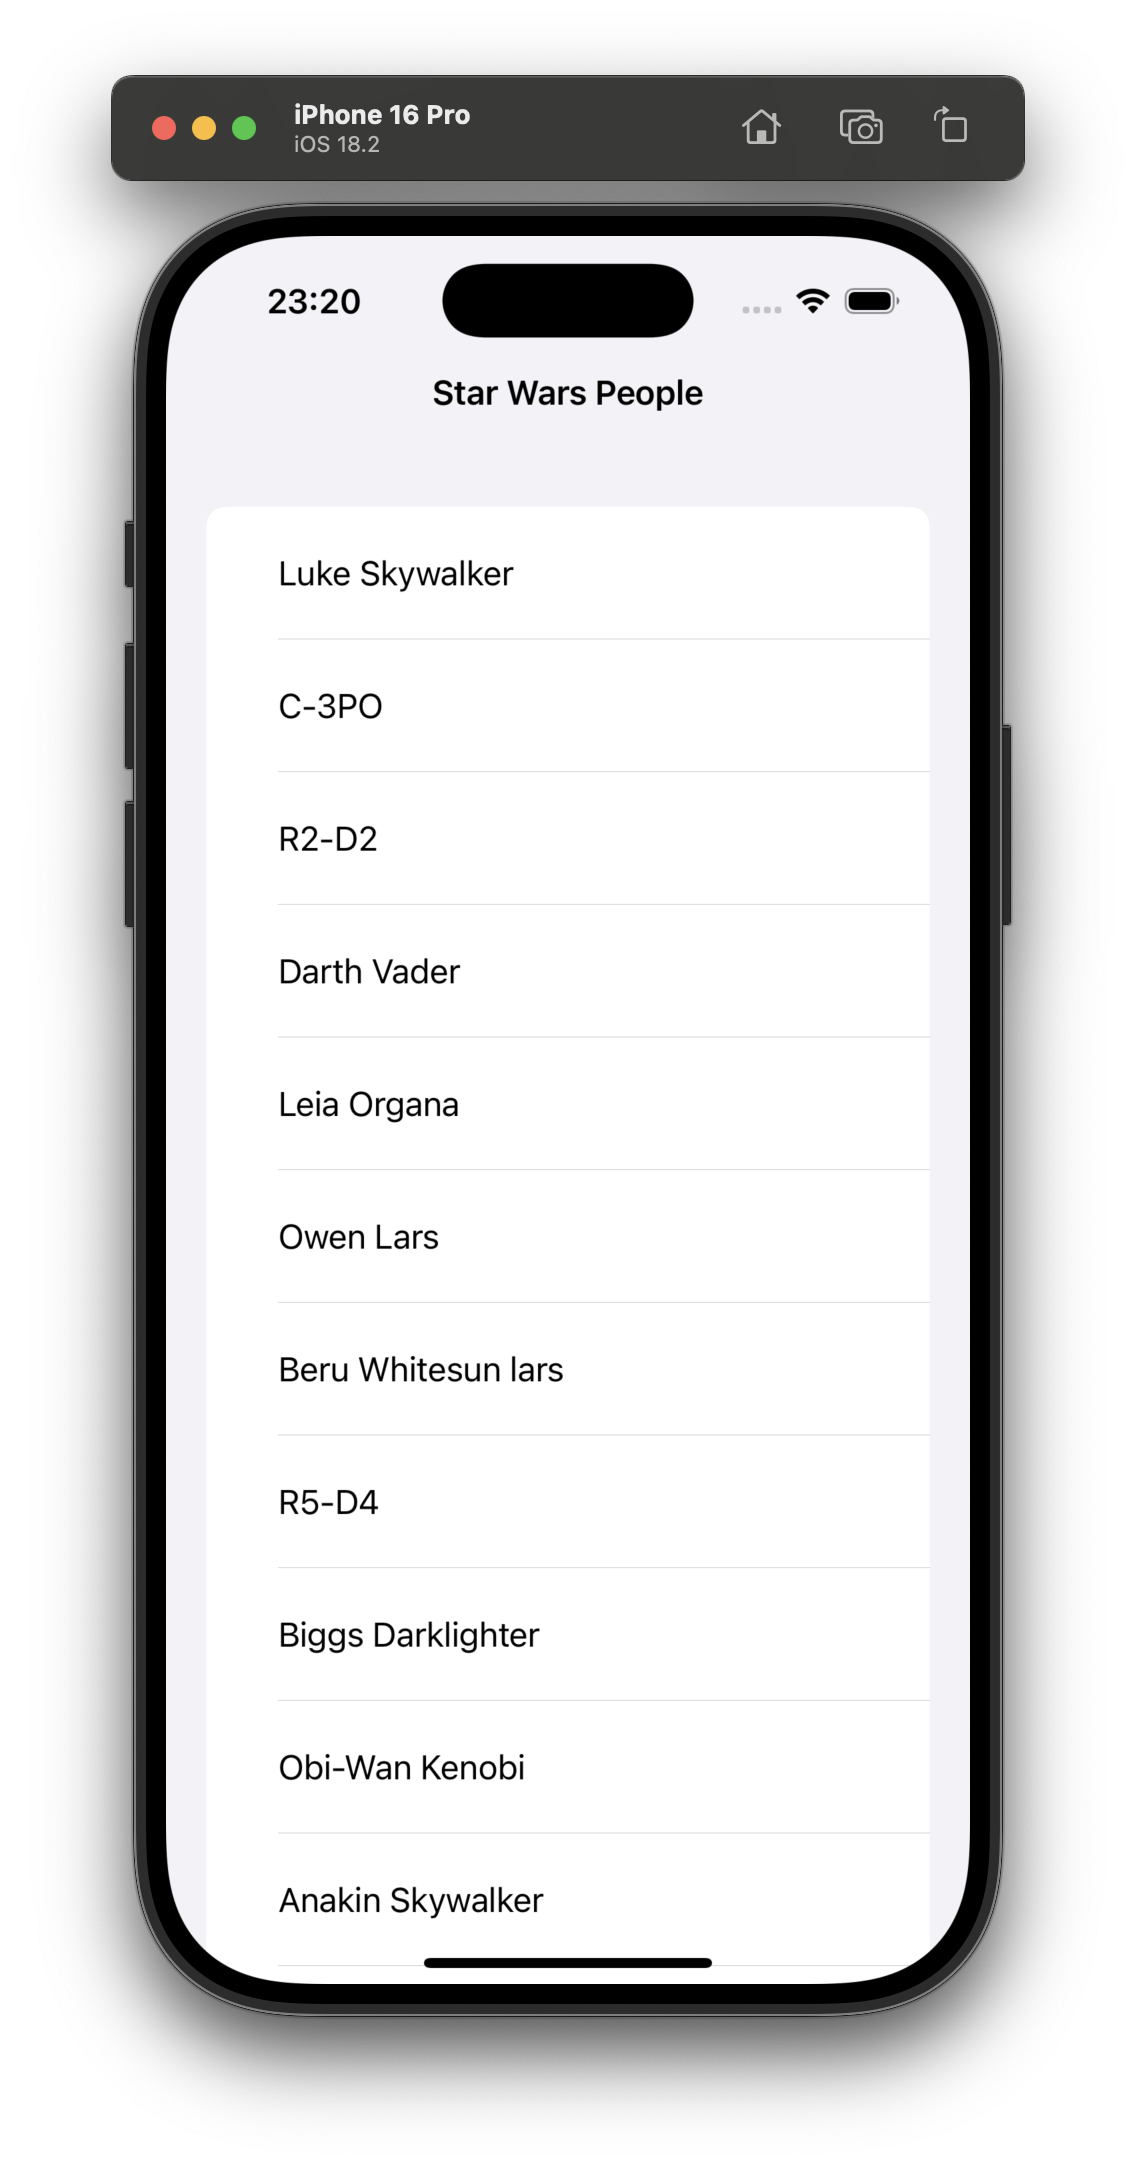
\includegraphics[width=0.4\textwidth]{ios_list.png}
    \caption{Экран со списком персонажей}
    \label{fig:list_screen}
\end{figure}


\begin{figure}[!htb]
    \centering
    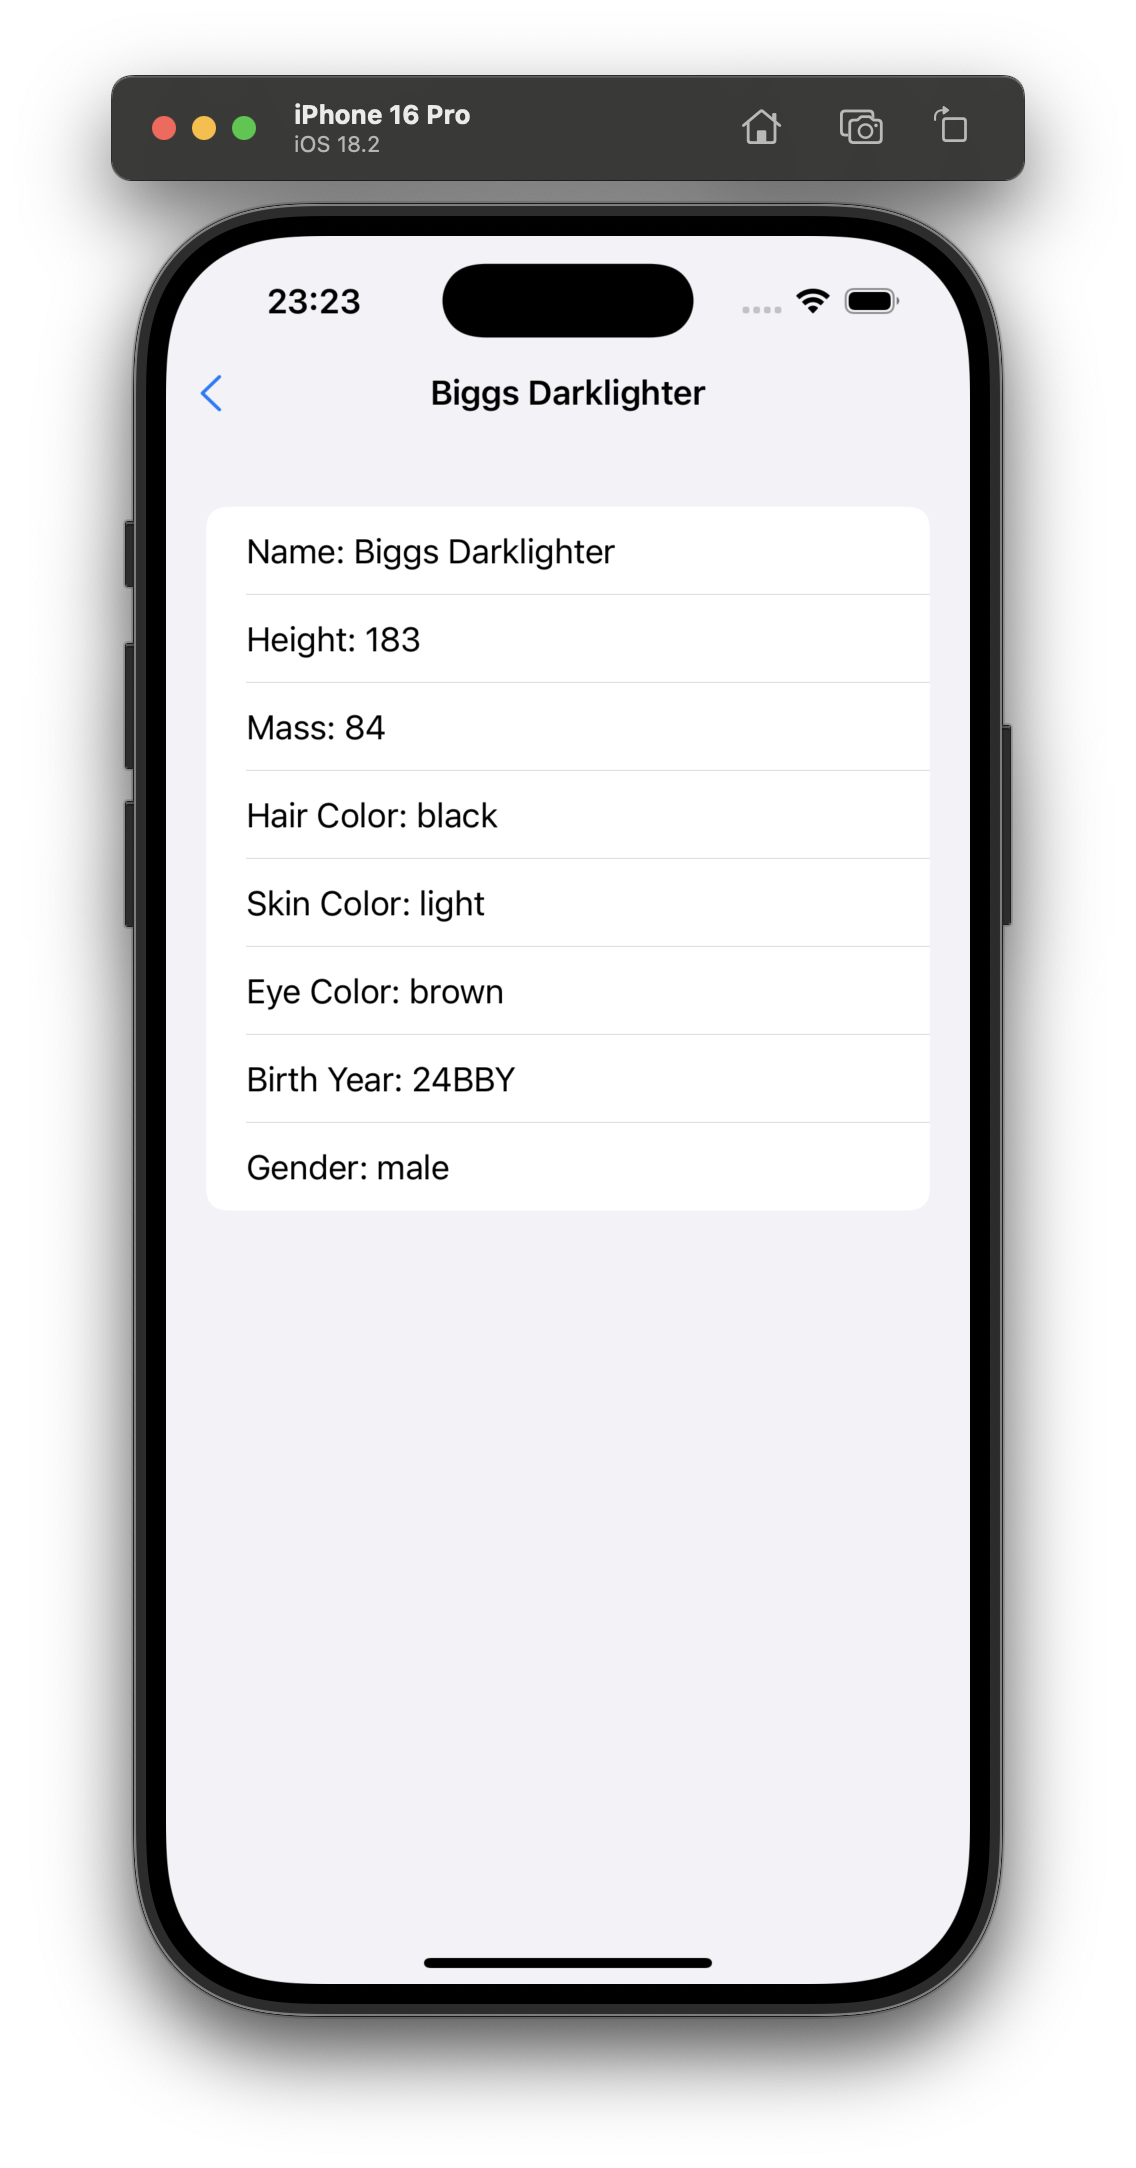
\includegraphics[width=0.4\textwidth]{ios_details.png}
    \caption{Экран с подробной информацией о персонаже}
    \label{fig:details_screen}
\end{figure}

\begin{figure}[!htb]
    \centering
    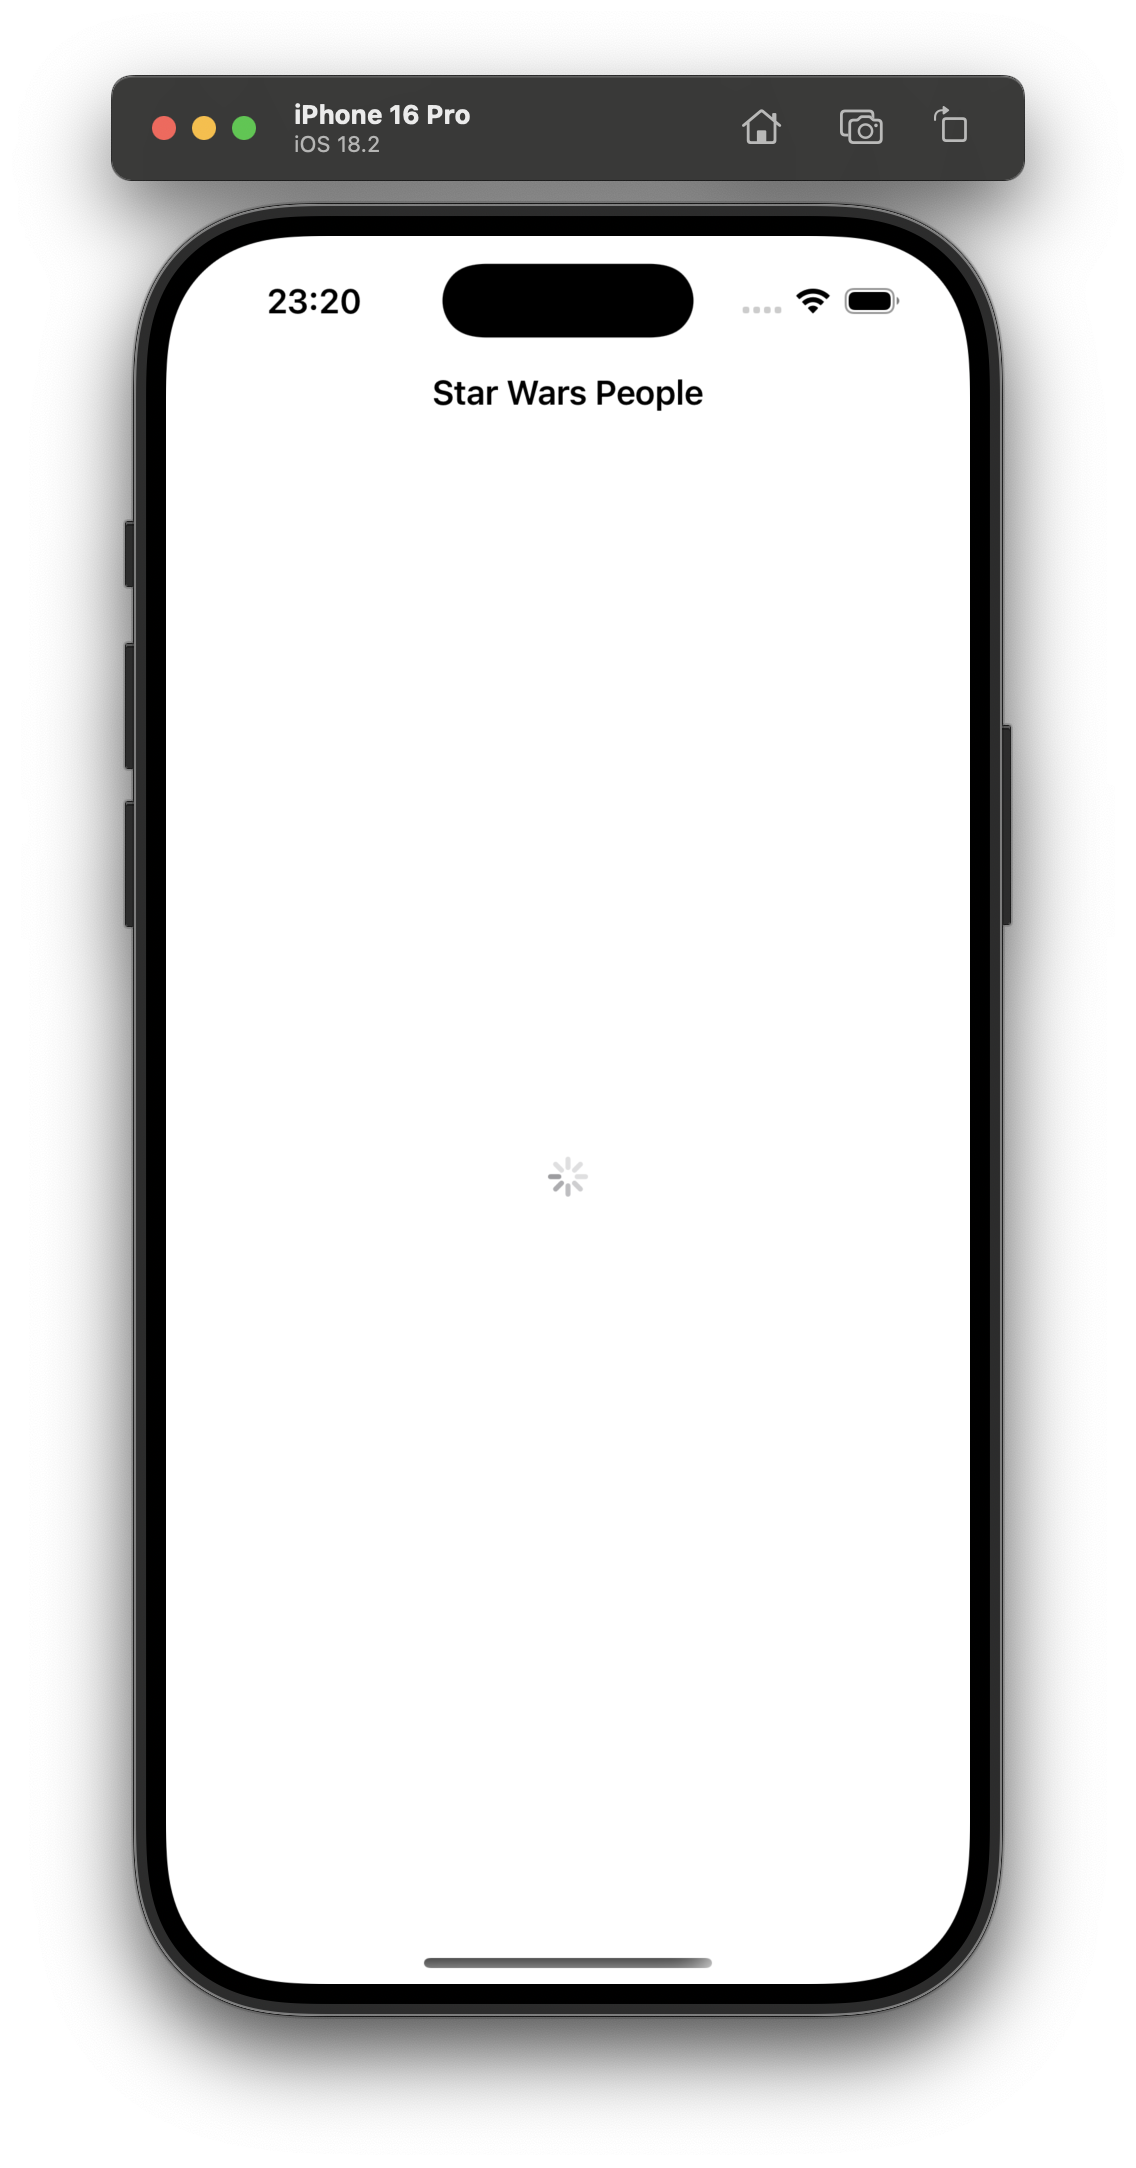
\includegraphics[width=0.4\textwidth]{ios_loading.png}
    \caption{Экран в состоянии загрузки}
    \label{fig:loading_screen}
\end{figure}

\begin{figure}[!htb]
    \centering
    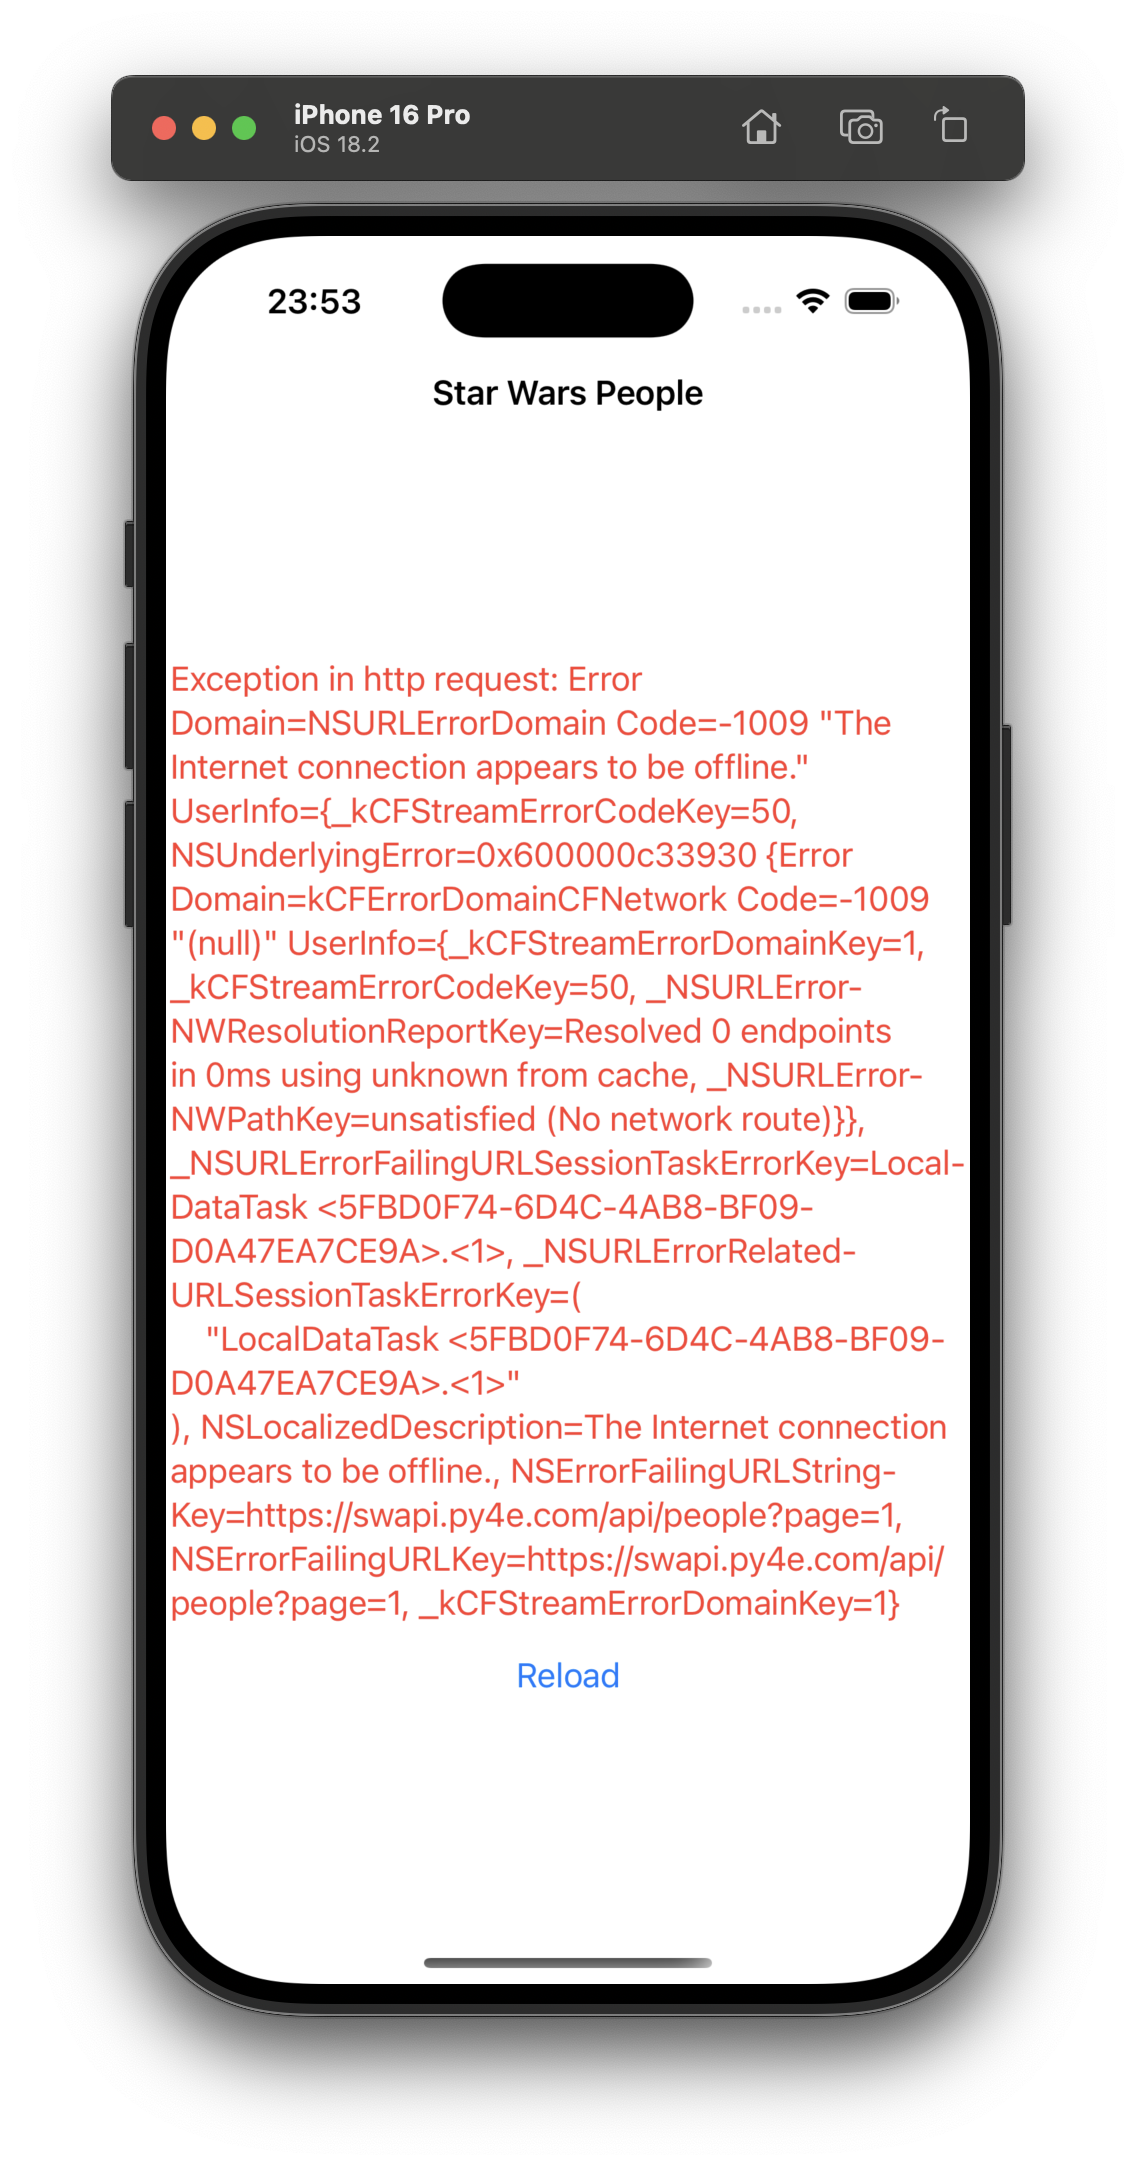
\includegraphics[width=0.4\textwidth]{ios_error.png}
    \caption{Экран в состоянии ошибки}
    \label{fig:error_screen}
\end{figure}

\subsection{Структура проекта}

Проект имеет стандартную для Kotlin Multiplatform архитектуру и состоит из двух основных модулей:

\begin{itemize}
    \item \texttt{shared}: Общий модуль, содержащий бизнес-логику, логику представления, сетевой слой и доменные модели. Код в этом модуле компилируется как для Android, так и для iOS.
    \item \texttt{iosApp}: Модуль, специфичный для платформы iOS, который содержит UI-слой, реализованный на SwiftUI, и обеспечивает интеграцию с общим кодом из модуля \texttt{shared}.
    \item \texttt{composeApp}: Модуль, отвечающий за пользовательский интерфейс на Jetpack Compose. Используется для приложений для платформ Android и Desktop, в данной курсовой работе не рассматривается.
\end{itemize}

Модуль \texttt{shared} внутри разделен на три логических слоя, что соответствует принципам чистой архитектуры:

\begin{itemize}
    \item \texttt{data}: Отвечает за получение данных из сети (с помощью Ktor) и их преобразование.
    \item \texttt{domain}: Содержит бизнес-сущности (модели) и интерфейсы репозиториев.
    \item \texttt{presentation}: Реализует логику представления с использованием MVIKotlin и управляет навигацией с помощью Decompose.
\end{itemize}

\subsection{Используемые технологии и библиотеки}

Для реализации проекта был выбран следующий стек технологий:

\begin{itemize}
    \item \textbf{Kotlin Multiplatform}: Основа для создания переиспользуемого кода между iOS и Android.
    \item \textbf{Decompose}: Библиотека для мультиплатформенной навигации и управления жизненным циклом компонентов. Она позволила реализовать всю навигационную логику в общем модуле \texttt{shared}.
    \item \textbf{MVIKotlin}: Реализация паттерна MVI для управления состоянием. Использовалась для создания предсказуемого и тестируемого потока данных.
    \item \textbf{Ktor}: Асинхронный сетевой фреймворк для выполнения HTTP-запросов к API.
    \item \textbf{Kotlinx.serialization}: Библиотека для сериализации и десериализации данных в формате JSON.
    \item \textbf{SwiftUI}: Декларативный фреймворк для построения UI на платформе iOS.
\end{itemize}

\subsection{Сетевое взаимодействие и загрузка данных}

Для выполнения сетевых запросов в общем модуле \texttt{shared} используется мультиплатформенная библиотека Ktor. Она позволяет один раз описать логику взаимодействия с API и переиспользовать ее на всех платформах. Настройка клиента Ktor происходит в общем коде, где устанавливаются базовый URL и настраивается сериализация JSON с помощью \texttt{kotlinx.serialization}, как показано в листинге \ref{lst:ktor_client}.

\begin{listing}[H]
\begin{minted}[frame=single,framesep=2mm,baselinestretch=1.2,fontsize=\small,linenos,breaklines]{kotlin}
// shared/data/network/HttpClient.kt
private val httpClient = HttpClient {
    install(ContentNegotiation) {
        json(Json {
            prettyPrint = true
            isLenient = true
            ignoreUnknownKeys = true
        })
    }
}
\end{minted}
\caption{Настройка HTTP-клиента Ktor}
\label{lst:ktor_client}
\end{listing}

Загрузка данных инкапсулирована в \texttt{Store}-компонентах (MVIKotlin), таких как \texttt{ListStore} и \texttt{DetailsStore}. Они инициируют асинхронную загрузку данных в \texttt{Bootstrapper} или \texttt{Executor}, используя корутины.

\subsection{Управление состоянием и пагинация}

Управление состоянием экранов реализовано с помощью MVIKotlin. Для каждого экрана (\texttt{ListComponent}, \texttt{DetailsComponent}) создан свой \texttt{Store}, который отвечает за обработку действий пользователя (\texttt{Intent}), выполнение бизнес-логики (\texttt{Executor}) и обновление состояния (\texttt{Reducer}).

Пагинация реализована на экране списка. Когда пользователь доходит до последнего видимого элемента, UI-слой на стороне iOS отправляет в \texttt{ListComponent} намерение \texttt{onLoadNextPageClicked}, как показано в листинге \ref{lst:swift_pagination_trigger}.

\begin{listing}[H]
\begin{minted}[frame=single,framesep=2mm,baselinestretch=1.2,fontsize=\small,linenos,breaklines]{swift}
// iosApp/ListView.swift
List {
    ForEach(model.items, id: \.url) { item in
        // ...
        .onAppear {
            if item == model.items.last {
                component.onLoadNextPageClicked()
            }
        }
    }
}
\end{minted}
\caption{Инициирование пагинации в SwiftUI}
\label{lst:swift_pagination_trigger}
\end{listing}

Это намерение обрабатывается в \texttt{ListStore}, который, в свою очередь, запускает загрузку следующей страницы данных, как показано в листинге \ref{lst:list_store_pagination}.

\begin{listing}[H]
\begin{minted}[frame=single,framesep=2mm,baselinestretch=1.2,fontsize=\small,linenos,breaklines]{kotlin}
// shared/presentation/list/ListStore.kt
private inner class ExecutorImpl : CoroutineExecutor<ListStore.Intent, Action, ListStore.State, Msg, Nothing>() {
    private var currentPage = 1

    override fun executeIntent(intent: ListStore.Intent) {
        when(intent) {
            is ListStore.Intent.LoadNextPage -> {
                if (!state().isLastPage && !state().isLoading) {
                    loadPage(currentPage + 1)
                }
            }
            // ...
        }
    }
}
\end{minted}
\caption{Обработка пагинации в ListStore}
\label{lst:list_store_pagination}
\end{listing}

\subsection{Обработка ошибок и интеграция с SwiftUI}

В случае ошибки при выполнении сетевого запроса \texttt{Store} перехватывает исключение и сохраняет сообщение об ошибке в своем состоянии, как показано в листинге \ref{lst:ktor_error_handling}.

\begin{listing}[H]
\begin{minted}[frame=single,framesep=2mm,baselinestretch=1.2,fontsize=\small,linenos,breaklines]{kotlin}
// shared/presentation/list/ListStore.kt
private fun loadPage(page: Int) {
    scope.launch(SupervisorJob()) {
        dispatch(Msg.Loading(true))
        peopleRepository.getPeople(page)
            .onSuccess {
                // ...
            }
            .onFailure {
                dispatch(Msg.Error(it.message ?: "Unknown Error"))
            }
    }
}
\end{minted}
\caption{Обработка ошибок сетевого запроса}
\label{lst:ktor_error_handling}
\end{listing}

Состояние из \texttt{Store} (включая ошибку) передается в \texttt{Component}, а затем в UI-слой iOS через обертку \texttt{ObservableValue}. SwiftUI-представление подписывается на изменения этого объекта и декларативно отображает либо данные, либо индикатор загрузки, либо сообщение об ошибке с кнопкой для повторной попытки (листинг \ref{lst:swift_error_handling}). Примеры состояний представлены на рисунках \ref{fig:list_screen}, \ref{fig:details_screen}, \ref{fig:loading_screen}, \ref{fig:error_screen}.

\begin{listing}[H]
\begin{minted}[frame=single,framesep=2mm,baselinestretch=1.2,fontsize=\small,linenos,breaklines]{swift}
// iosApp/ListView.swift
ZStack {
    if let error = model.error, !model.isLoading {
        VStack(spacing: 16) {
            Text(error)
                .foregroundColor(.red)
            Button("Reload", action: component.onReloadClicked)
        }
    } else {
        // ... отображение списка
    }

    if model.items.isEmpty, model.isLoading {
        ProgressView()
    }
}
\end{minted}
\caption{Отображение состояния ошибки в SwiftUI}
\label{lst:swift_error_handling}
\end{listing}

Этот подход позволяет полностью инкапсулировать логику загрузки данных и обработки ошибок в общем \texttt{shared}-модуле, оставляя для iOS-приложения только задачу отображения готового состояния.

\section{Анализ и выводы}

На основе практической реализации и теоретического обзора был проведен анализ выбранного архитектурного подхода — связки MVIKotlin и Decompose — в контексте iOS-ориентированного проекта на Kotlin Multiplatform.

\subsection{Сильные стороны}

Выбранный стек продемонстрировал ряд значительных преимуществ, ключевых для мультиплатформенной разработки:

\begin{itemize}
    \item Максимальное переиспользование кода. Вся бизнес-логика, логика представления (управление состоянием) и даже навигация были вынесены в общий модуль \texttt{shared}. Это сокращает дублирование кода и упрощает синхронизацию версий приложения для разных платформ.
    \item Масштабируемость. Компонентная модель Decompose позволяет легко добавлять новые экраны и потоки, изолируя их логику. Такой подход предотвращает разрастание классов и смешивание ответственности, в отличие от потенциальной проблемы «Massive ViewModel» в классическом MVVM.
    \item Нативная производительность. Поскольку UI-слой для каждой платформы остается полностью нативным (SwiftUI для iOS), приложение сохраняет высокую производительность и отзывчивость, свойственную нативным решениям. Общая логика компилируется в нативный код, не создавая дополнительных издержек.
    \item Платформонезависимая отладка. Бизнес-логику и логику представления можно разрабатывать, тестировать и отлаживать в общем модуле, используя, например, desktop-запуск. Это позволяет вести основную часть разработки, не имея под рукой iOS-устройства или MacBook, что значительно ускоряет и упрощает процесс.
    \item Предсказуемость и тестируемость. Паттерн MVI обеспечивает строгий однонаправленный поток данных, что делает поведение приложения предсказуемым, а отладку — прозрачной. Логика обновления состояния инкапсулирована в чистых функциях-редьюсерах, которые легко покрываются юнит-тестами.
\end{itemize}

\subsection{Слабые стороны}

Несмотря на весомые преимущества, у подхода есть и недостатки:

\begin{itemize}
    \item Высокий порог входа. Для эффективного использования стека MVIKotlin + Decompose разработчикам, особенно привыкшим к классическому MVVM, требуется время на освоение новых концепций и библиотек.
    \item Увеличенный объем шаблонного кода. Реализация каждого экрана требует описания \texttt{State}, \texttt{Intent} и \texttt{Store}, что для простых случаев может показаться избыточным по сравнению с лаконичностью MVVM.
    \item Интеграционный слой. Для связи общего кода с нативным UI (SwiftUI) требуется создание дополнительного слоя-адаптера, что добавляет сложности, хотя и решается универсальными обертками.
\end{itemize}

\section{Заключение}

Выбранный архитектурный стек MVIKotlin + Decompose является мощным и стратегически верным решением для средних и крупных KMP-проектов, где важны долгосрочная поддержка, масштабируемость, максимальное переиспользование кода и строгая архитектура. Он идеально подходит для команд, готовых инвестировать время в изучение подхода, чтобы получить предсказуемую и легко тестируемую кодовую базу.

Для небольших проектов или прототипов, где скорость разработки является ключевым фактором, а команда не знакома с MVI, более прагматичным выбором может стать адаптация MVVM. Однако в таком случае вопросы навигации и межэкранного взаимодействия придется либо решать отдельно для каждой платформы, что снизит объем переиспользуемого кода, либо написать собственное решение \texttt{ViewModel} поверх Decompose, не используя MVIKotlin, что потребует от разработки изучения данного фреймворка.


\end{document}
